\section{Classifier Decision Functions}
\begin{multicols}{2}

Many classifiers in scikit learn can provide information about the uncertainty associated with a particular prediction either by using the \textbf{decision function} method or the \textbf{predict proba} method. 

\subsection{Decision function method}

When given a set of test points, the decision function method provides for each one a classifier score value that indicates how confidently classifier predicts the positive class. So there will be large magnitude positive scores for those points, or it predicts a negative class, there'll be large magnitude negative scores for negative points. 

Here's an example in the notebook showing the first few instances from our classification problem using a logistic regression classifier. We can see the instances in the negative class often have large magnitude negative scores. And indeed the instances in the positive class has positive scores from the logistic regression classifier. 

\subsection{Predict proba function}

Likewise, the \texttt{predict_proba} function provides \emph{predicted probabilities} of class membership. 

Typically a classifier would choose the more likely class. That is in a binary classifier, the class with probability greater than 50\%. 

\subsection{Decision threshold}

Adjusting this decision threshold affects the prediction of the classifier. A higher threshold means that a classifier has to be more confident in predicting the class. For example, we might predict class one only if the estimated probability of class one was over 70\%. And this results in a more conservative classifier. 

Here's an example of getting these prediction probabilities for the test instances for the same logistic regression classifier. 

You can see that many entries with a positive label of one, have a high probability like 0.995. While many negative label instances have a very low prediction probability. 

\textbf{Note} that \emph{not all} models provide useful probability estimates of this type. For example, a model that was over-fit to a trending set, might provide overly optimistic high probabilities that were in fact not accurate. 

Now, we can use these decision scores or prediction probabilities for getting more complete evaluation picture of a classifiers performance. For a particular application, we might pick a specific decision threshold depending on whether we want the classifier to be more or less conservative about making false-positive or false-negative errors. 

It might not be entirely clear when developing a new model, what the right decision threshold would be, and how that choice will affect evaluation metrics like precision and recall. So instead, what we'll do is, look at how classifier performs for all possible decision thresholds. 

This example shows how that works. On the left here is a list of test instances with their true label and classifier score. 

\begin{center}
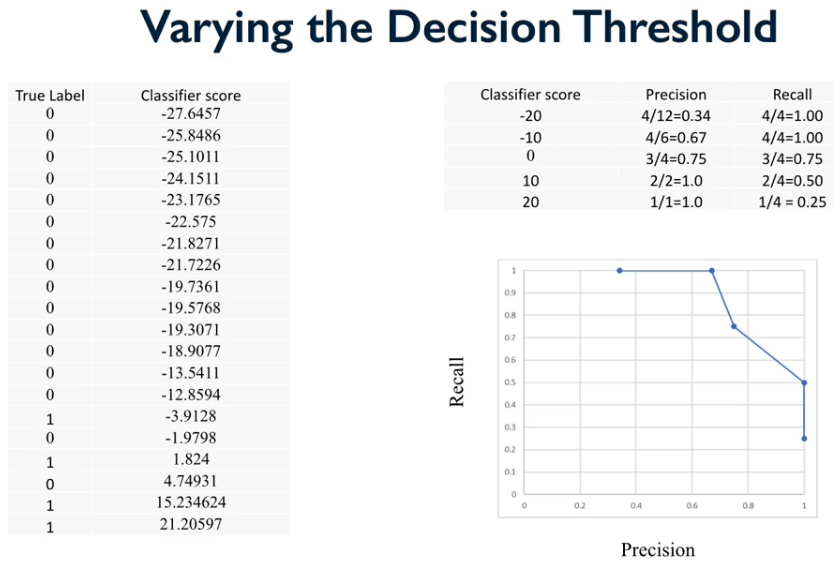
\includegraphics[width=\linewidth]{img/Varying-Decision-Threshold.png} 
\end{center}

If we set a decision threshold, then all the instances above that line, for example if we set the decision threshold to be -20 here. 

Then, all the instances above the line are below the threshold of -20. So -20 or less and all the instances in this direction are above the threshold of -20. And so the ones below the threshold will be predicted to be in the- class. 

And the ones above the threshold will be predicted to be in the + class. 

So, if we pick the specific threshold, so in this case, -20. And we partition the test points in this way. We can compute partition and recall for the points that are predicted to be in the positive class. So in this case, we have 12 instances here, 12 total instances. 

They're being predicted as positive and only four of them, this one, this one, this one, and this one are actually positive and so the precision here is 4 divided by 12 or approximately 0.34. 

The recall on the other hand, there are four positive labeled instances in the whole set of test examples here and we've found all of them with this particular threshold setting. So the recall here is 4 out of 4, we found all four positive labeled examples. And so, for this particular threshold of -20, we can obtain precision on re cost score for that threshold. 

Let's pick a different threshold let's look at what happened when the threshold is -10? Right here, so again anything below this line is treated and has a higher value than -10 here, so those would be treated as + predictions. 

Things above the line have a score below -10, so these would be predicted to be 

And again, we can compute a precision and recall for this decision threshold setting, and we can see here that there are a total of six instances in the + prediction class. Of which four are actually of the positive class, and so the precision here is 4 over 6 or about 0.67. And again, the recall here is going to be 4 out of 4, and it's going to be 1.0. Again, so that corresponds to this point in the table over here. And then as were computing these different precision and recalls for different Thresholds. We can also plot them on this precision recall chart. So the first pair of precision recall numbers that I got, 0.34 and 1.0, we can plot on this point in precision recall space. The second example, so this was for the threshold of -20. 

When the threshold was -10, we got precision of .67 and a recall of 1 corresponding to this point that we can plot. 

And so you can see that if we do this for a number of other thresholds, for example the threshold of 0, we'll get a precision of 0.75. And a recall of 0.75 that corresponds to this point. 

And in that choice of decision threshold. And we can keep doing that for different thresholds. And we actually are plotting a series of points through the space which we can be connected at as a curve. 

And so in this way, we can get a more complete picture by varying the threshold of how the precision and recall of the result and classifier output changes as a function of the decision threshold. 

And this resulting chart here is called a precision recall curve and we'll look at it in more detail next. 

\end{multicols}